\section{Evaluation Results}\label{result}

This section presents quantitative evaluation results of the proposed adaptive-precision ADC 
designs, including a column-parallel Single-Slope (SS) ADC and a column-parallel successive 
approximation register (SAR)/SS ADC. Both ADC designs are implemented using TSMC 65nm processing,
and simulated in Virtuoso’s AMS Environment. Circuit power consumption is collectively estimated
based on the average transient current of different ADC modules given one complete sampling and 
conversion period. Power savings are then estimated by comparing the power consumption of the
low-precision conversion mode against that of the high-precision conversion mode. 

Specifically, the detailed power-breakdown and power-saving results of the proposed SS and SAR/SS ADC designs are presented in \ref{SS power} and \ref{SAR power}. And the key design characteristics are summarized in \ref{summary}, with a comparison between our work and previous reported configurable ADCs.

\subsection{Power-scaling Performance of the SS ADC Design}\label{SS power}
%Table~\ref{tab1} summarizes the key design characteristics of the SS ADC design. Considering a 
%$512\times512$ pixel array, the frame rate is 162fps.  The SNDR of the SS ADC is 23.83/46.64 dB, 
%which means the ENOB is 3.67/7.46 bits.  

Fig.~\ref{SSresults1} shows the detailed power-breakdown results of the SS ADC design,
which demonstrates that the power consumption of the SS ADC design is mainly contributed by 
the column-parallel comparators and the output buffer of the ramp generator, both of which 
can be effectively regulated via power gating for low-power conversion. The peripheral circuits include a bandgap and voltage divider, level-shift circuits and global buffers.

The power-saving results are also presented in Fig.~\ref{SSresults2}, where the annotated power consumption is measured and divided by column. It shows that the total power consumption of the low-precision conversion mode is 40.8uW/column, and the power consumption of the high-precision conversion mode is 76.2uW/column. 
Compared to the high-precision conversion mode, the low-precision conversion mode can reduce 
the power consumption approximately 50\%, which is contributed by the power-gating-regulated comparators and buffer.

\iffalse
\begin{table}[htbp]
	\caption{PERFORMANCE OF THE SS ADC DESIGN}
	\begin{center}
		\begin{tabular}{|c|c|}
			\hline
			\textbf{Prameter}& \textbf{Value} \\
			\hhline{|==|}
			\textbf{Process}& 65nm \\
			\hline 
			\textbf{Supply voltage}& 2.5/1.2 V \\
			\hline
			\textbf{Clock Frequency}&	25MHz \\
			\hline
			\textbf{Architecture}&	SS \\
			\hline
			\textbf{Quantization bits}&	4/8 bits\\
			\hline
			\textbf{Conversion time}&	12.04us \\
			\hline
			\textbf{Number of parallel columns}&	512 \\
			\hline
			\textbf{Throughput (samples per second)}&	42.5M \\ 
			\hline
			\textbf{Power (per column)}&	40.8/76.2 uW \\
			\hline
			\textbf{SNDR}& 23.83/46.64 dB@ 8.44 kHz\\
			\hline
			\textbf{ENOB}& 3.67/7.46 bits\\
			\hline
			\textbf{FOM$^{\mathrm{a}}$}& 38.59/5.21 pJ/step\\
			\hline
			\multicolumn{2}{l}{$^{\mathrm{a}}\textbf{FOM}=(\textbf{Power}\ast \textbf{Conversion}\ \textbf{time})/2^{\textbf{ENOB}}$ }	    
		\end{tabular}
		\label{tab1}
	\end{center}
\end{table}
\fi

\begin{figure}[htbp]
	\centerline{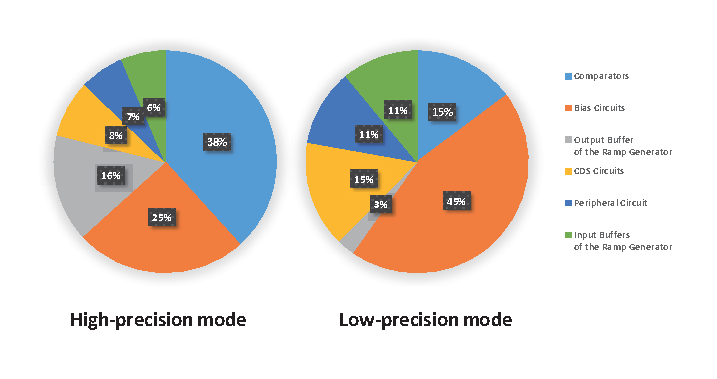
\includegraphics[width=3.5in]{./Figures/SSResults1.eps}}
	\caption{Power-breakdown results of the SS ADC design.}
	\label{SSresults1}
\end{figure}

\begin{figure}[htbp]
	\centerline{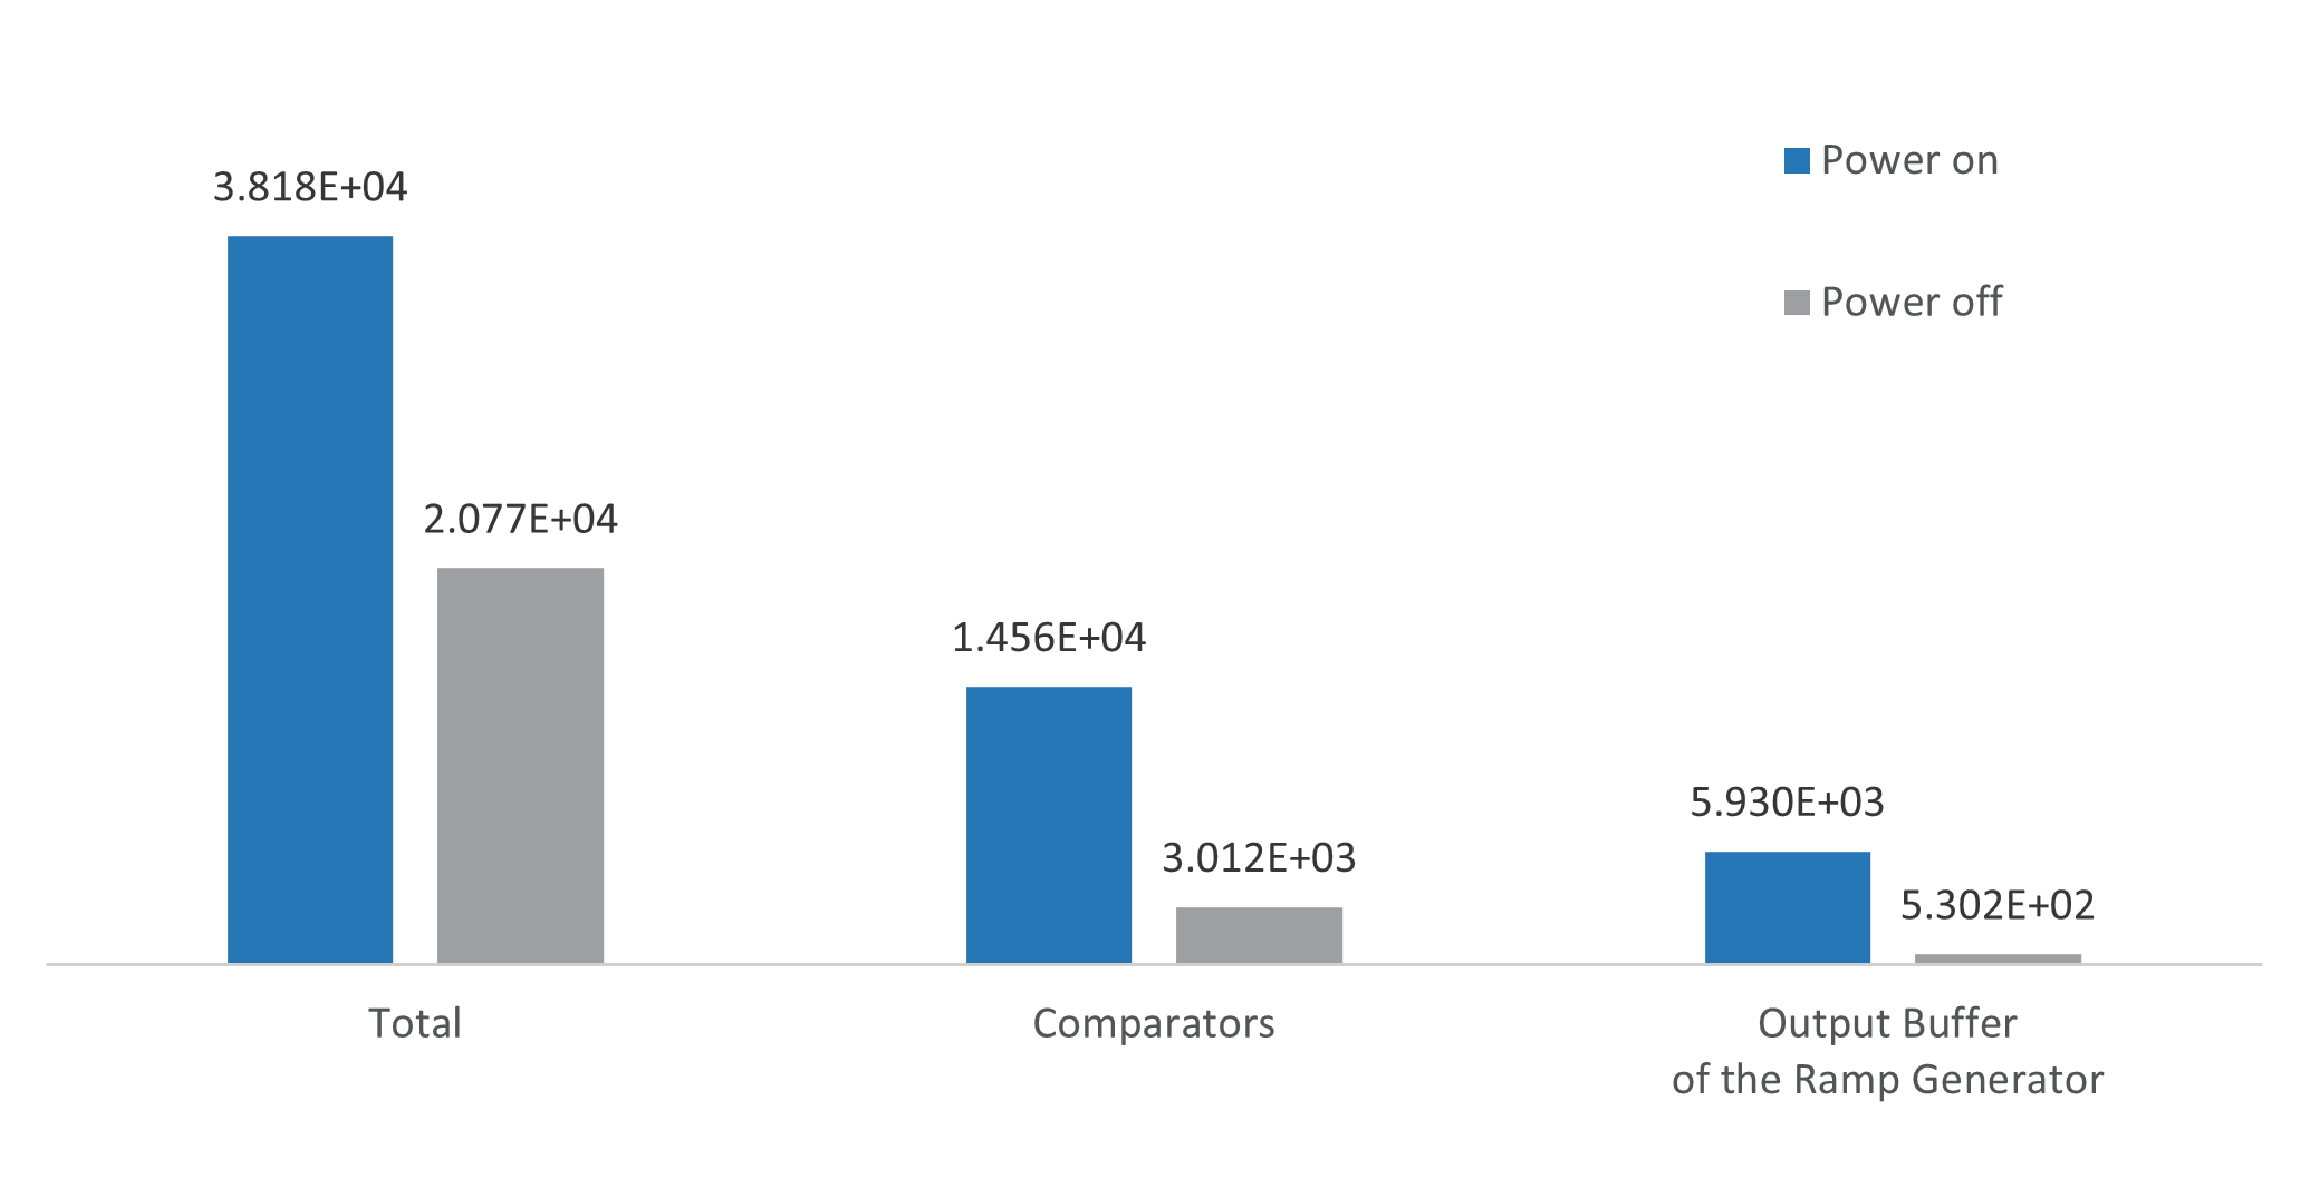
\includegraphics[width=3.5in]{./Figures/SSResults2.eps}}
	\caption{Power-saving results of the SS ADC design.}
	\label{SSresults2}
\end{figure} 

\subsection{Evaluation of the SAR/SS ADC design}\label{SAR power}

%Table~\ref{tab2} summarizes the key design characteristics of the SAR/SS ADC design, for which 
%we consider the same setup as that of the SS ADC. Since fewer steps are required in the SAR/SS ADC 
%design, 1 step is equivalent to 2 clock periods. The SNDR is 24.25/57.87 dB and the ENOB is 3.74/9.32 bits, 
%which is inline with the design specifications. 

Fig.~\ref{SARresults1} shows the detailed power-breakdown results of the SAR/SS ADC design, which 
demonstrates that the power consumption of the SAR/SS ADC design is mainly contributed by the column-parallel buffers of the reference voltages in the sub-ADCs, and power gating can effectively minimize the power consumption of these 
power-dominant components. 

The power-saving results are also presented in Fig.~\ref{SARresults2}, showing that the total power consumption of the SAR/SS ADC design is 256.1uW/column for the high-precision conversion mode and 137.1uW/column for the low-precision conversion mode. 
Compared to the high-precision conversion mode, the low-precision conversion mode can reduce the power consumption approximately 50\%.

\iffalse
\begin{table}[htbp]
	\caption{PERFORMANCE OF THE SAR/SS ADC DESIGN}
	\begin{center}
		\begin{tabular}{|c|c|}
			\hline
			\textbf{Prameter}& \textbf{Value} \\
			\hhline{|==|}
			\textbf{Process}& 65nm \\
			\hline 
			\textbf{Supply voltage}& 2.5/1.2 V \\
			\hline
			\textbf{Clock Frequency}&	20MHz \\
			\hline
			\textbf{Architecture}&	SAR/SS \\
			\hline
			\textbf{Quantization bits}&	4/10 bits \\
			\hline
			\textbf{Conversion time (us)}&	10.1us \\
			\hline
			\textbf{Number of parallel columns}&	512 \\
			\hline
			\textbf{Throughput (samples per second)}&	50.7M \\ 
			\hline
			\textbf{Power (per column)}&	137.1/256.1 uW \\
			\hline
			\textbf{SNDR}& 24.25/57.87 dB@ 10.06 kHz \\
			\hline
			\textbf{ENOB}& 3.74/9.32 bits \\
			\hline
			\textbf{FOM$^{\mathrm{a}}$}& 103.64/4.05 pJ/step\\
			\hline
			\multicolumn{2}{l}{$^{\mathrm{a}}\textbf{FOM}=(\textbf{Power}\ast \textbf{Conversion}\ \textbf{time})/2^{\textbf{ENOB}}$ }	    
		\end{tabular}
		\label{tab2}
	\end{center}
\end{table}
\fi

\begin{figure}[htbp]
	\centerline{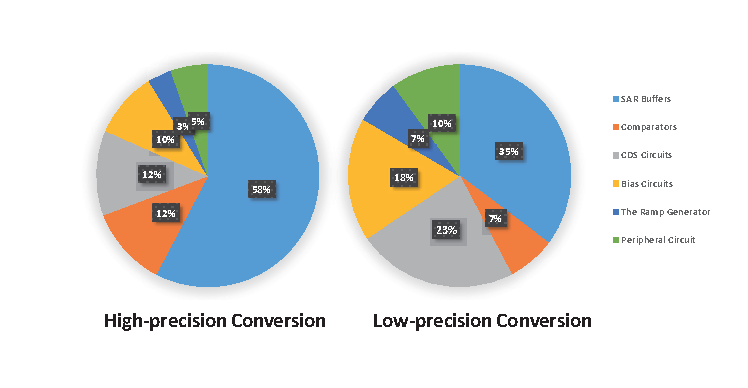
\includegraphics[width=3.5in]{./Figures/SARResults1.eps}}
	\caption{Power-breakdown results of the SAR/SS ADC design.}
	\label{SARresults1}
\end{figure} 

\begin{figure}[htbp]
	\centerline{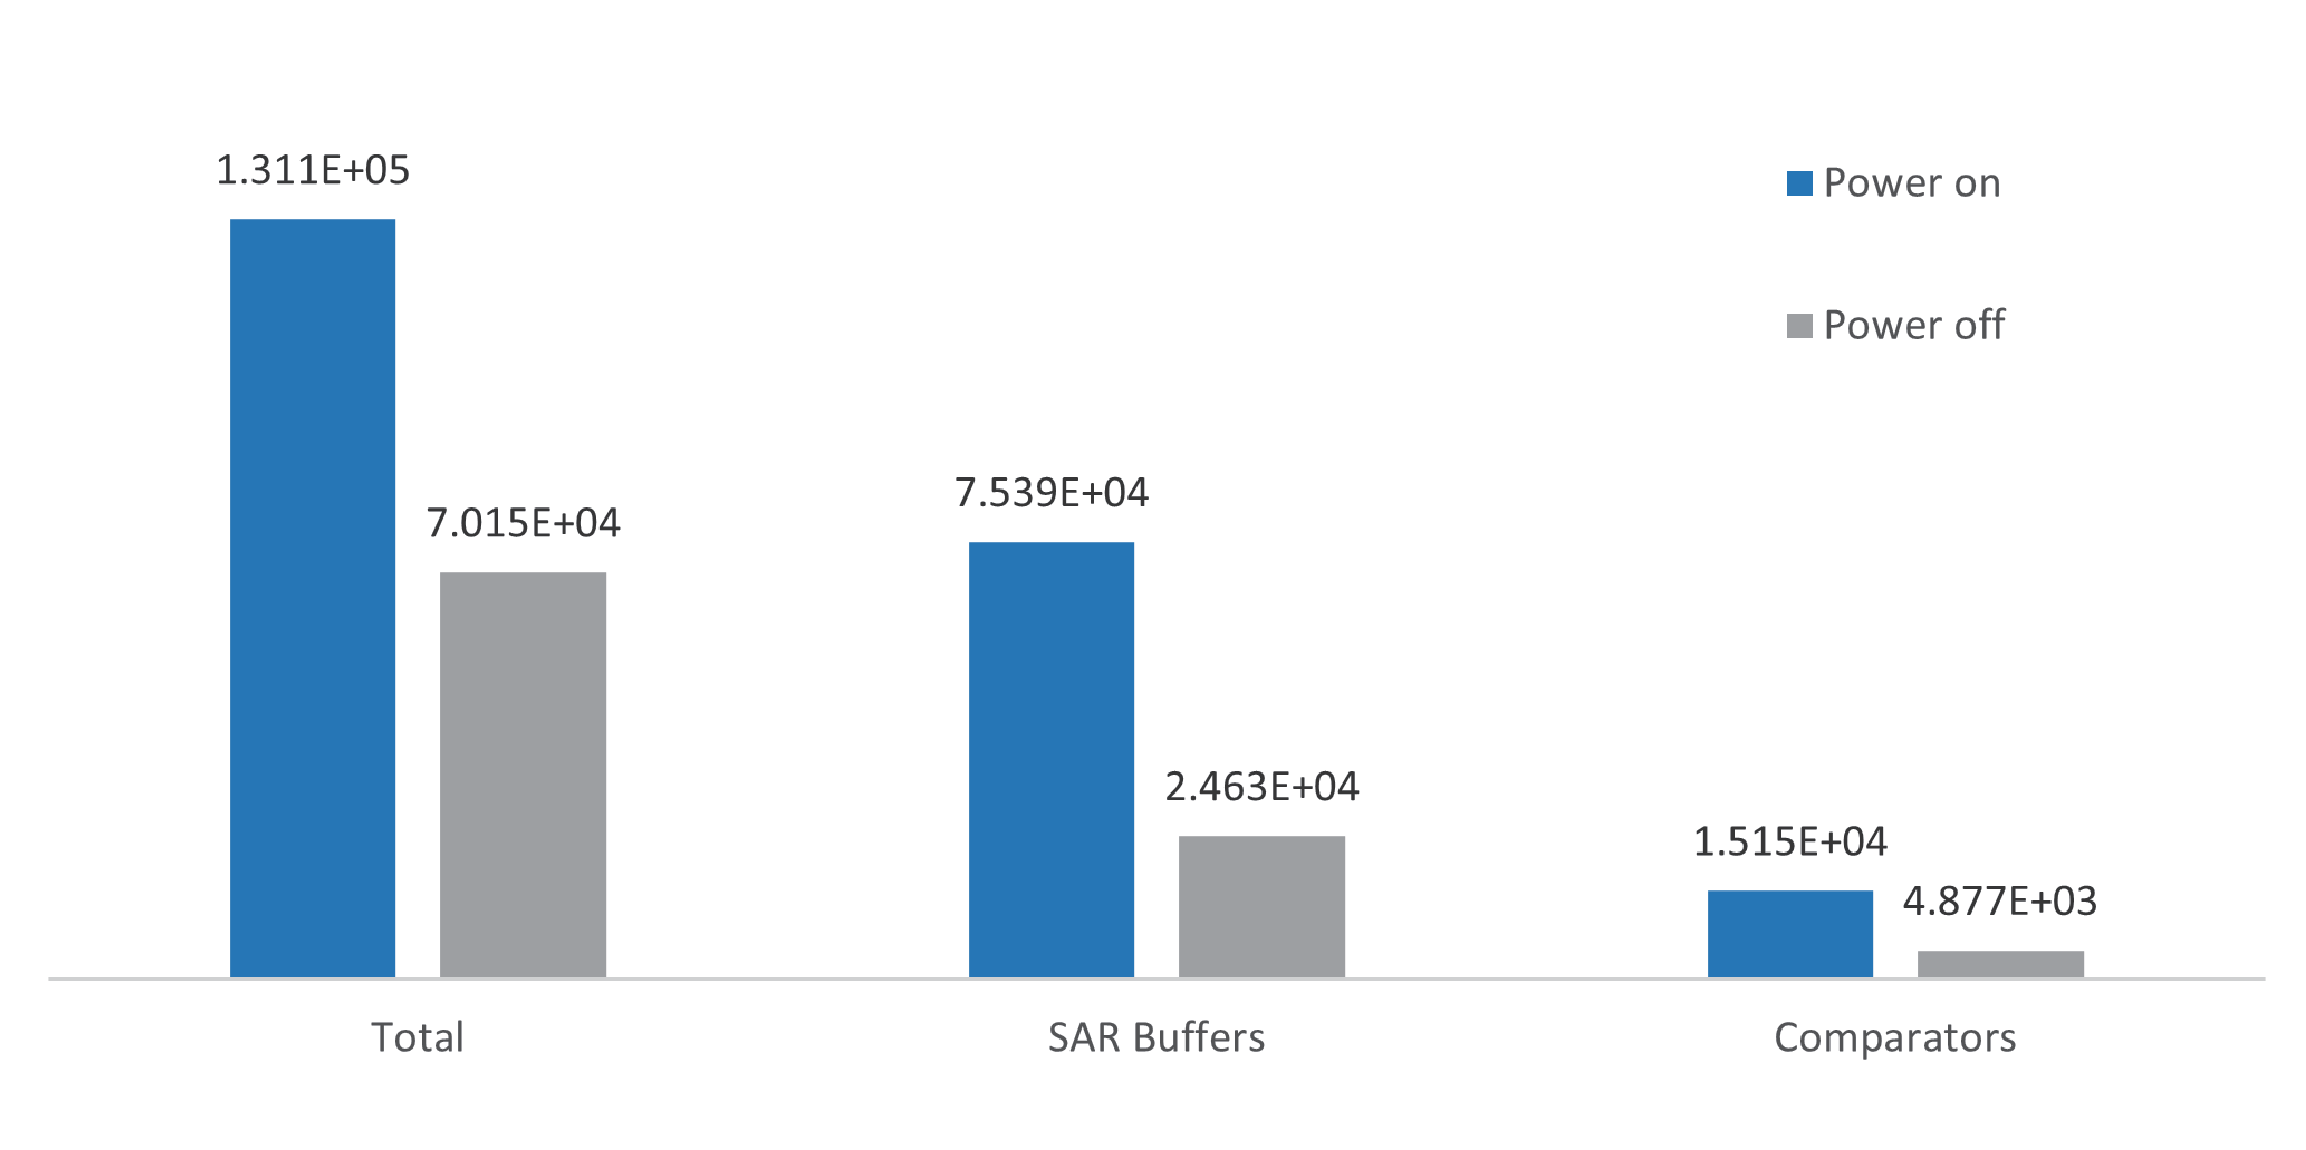
\includegraphics[width=3.5in]{./Figures/SARResults2.eps}}
	\caption{Power-saving results of the SAR/SS ADC design.}
	\label{SARresults2}
\end{figure} 

\subsection{Performance Summary and Comparison}\label{summary}

Table~\ref{tab1} summarizes the key characteristics of the proposed SS and SAR/SS ADC designs.
And a comparison with previous reported configurable ADCs is also provided. 
We take the precision-adaptive SAR ADCs into comparison because on the one hand they have similar precision and sampling rate configurations to our design, on the other hand, SAR ADCs are also applicable to column-parallel image processing given a relatively loose area constraint.

It is highlighted that our design achieves better power-scaling performance than previous works. And the presented power-scaling percents of the SAR ADCs can actually be worse because in these works only the power consumption of the core ADC circuit is measured, while we have analysed the power consumption of the whole proposed implementation, including the bandgap, voltage divider, bias circuits and reference buffers. Therefore, with fairly considering the peripheral fixed parts of energy, the power-scaling performance of our design can definitely be more competitive.

It is noted that the overall power consumption of the proposed implementation is relatively large with high supply voltages. However, since our design studies are targeting to exploit the power-scaling capabilities with applying reasonable power gating strategies, rather than shrinking the power consumption as more as possible for the ADCs equipped with fixed-precision, instructive power-saving effectiveness is still demonstrated.

\begin{table*}[htbp]
	\caption{PERFORMANCE AND COMPARISON}
	\begin{center}
		\begin{tabular}{|c|c|c|c|c|c|c|c|c|}
			\hline
			\textbf{}& \multicolumn{2}{|c|}{\cite{zhu_6--10-bit_2015}} & \multicolumn{2}{|c|}{\cite{yip_resolution-reconfigurable_2013}} & \multicolumn{4}{|c|}{This work} \\
			\hhline{|=========|}
			%\iffalse
			\textbf{Process}& \multicolumn{2}{|c|}{180nm} & \multicolumn{2}{|c|}{65nm} & \multicolumn{4}{|c|}{65nm} \\
			\hline 
			\textbf{Supply voltage}& \multicolumn{2}{|c|}{0.6V} & \multicolumn{2}{|c|}{0.4V-1V} & \multicolumn{4}{|c|}{2.5V(Analog), 1.2V(Digital)} \\
			\hline
			
			%\textbf{Clock Frequency}&	20MHz \\
			%\hline
			\textbf{Architecture}& \multicolumn{2}{|c|}{SAR} & \multicolumn{2}{|c|}{SAR} & \multicolumn{2}{|c|}{SS} & \multicolumn{2}{|c|}{SAR/SS}\\
			\hline
			\textbf{Precison(bits)} & 8 & 10 & 6 & 10 & 4 & 8 & 4 & 10 \\
			\hline
			\textbf{Sampling rate(Hz)}& \multicolumn{2}{|c|}{100K} & \multicolumn{2}{|c|}{20K} & \multicolumn{2}{|c|}{83K} & \multicolumn{2}{|c|}{99K} \\
			\hline
			%\textbf{Number of parallel columns}&	512 \\
			%\hline
			%\textbf{Throughput (samples per second)}&	50.7M \\ 
			%\hline
			\textbf{SNDR(dB)} & 47.4 & 60.5 & 36.6 & 55.0 & 23.83 & 46.64 & 24.25 & 57.87 \\
			\hline
			\textbf{ENOB(bits)}& 7.58 & 9.76 & 5.79 & 8.84 & 3.67 & 7.46 & 3.74 & 9.32 \\
			\hline
			\textbf{Power consumption}& 0.32$\mu$W & 0.52$\mu$W &  0.116$\mu$W & 0.226$\mu$W & 40.8$\mu$W & 76.2$\mu$W & 137.1$\mu$W & 256.1$\mu$W\\
			\hline
			\textbf{Power-scaling performance}& 62\% & 100\% & 56\% & 100\% & \textbf{54}\% & 100\% & \textbf{54}\% & 100\% \\
			\hline
			%\fi
			%\textbf{FOM$^{\mathrm{a}}$}& 103.64/4.05 pJ/step\\
			%\hline
			%\multicolumn{2}{l}{$^{\mathrm{a}}\textbf{FOM}=(\textbf{Power}\ast \textbf{Conversion}\ \textbf{time})/2^{\textbf{ENOB}}$ }	    
		\end{tabular}
		\label{tab1}
	\end{center}
\end{table*}